\documentclass[border=10pt]{standalone}
\usepackage[svgnames]{xcolor}
\usepackage{amsmath}
\usepackage{pgfplots}
\pgfplotsset{compat=newest}
\usepackage[sfdefault]{FiraSans}
\usepackage{FiraMono}
\renewcommand*\familydefault{\sfdefault}
\begin{document}
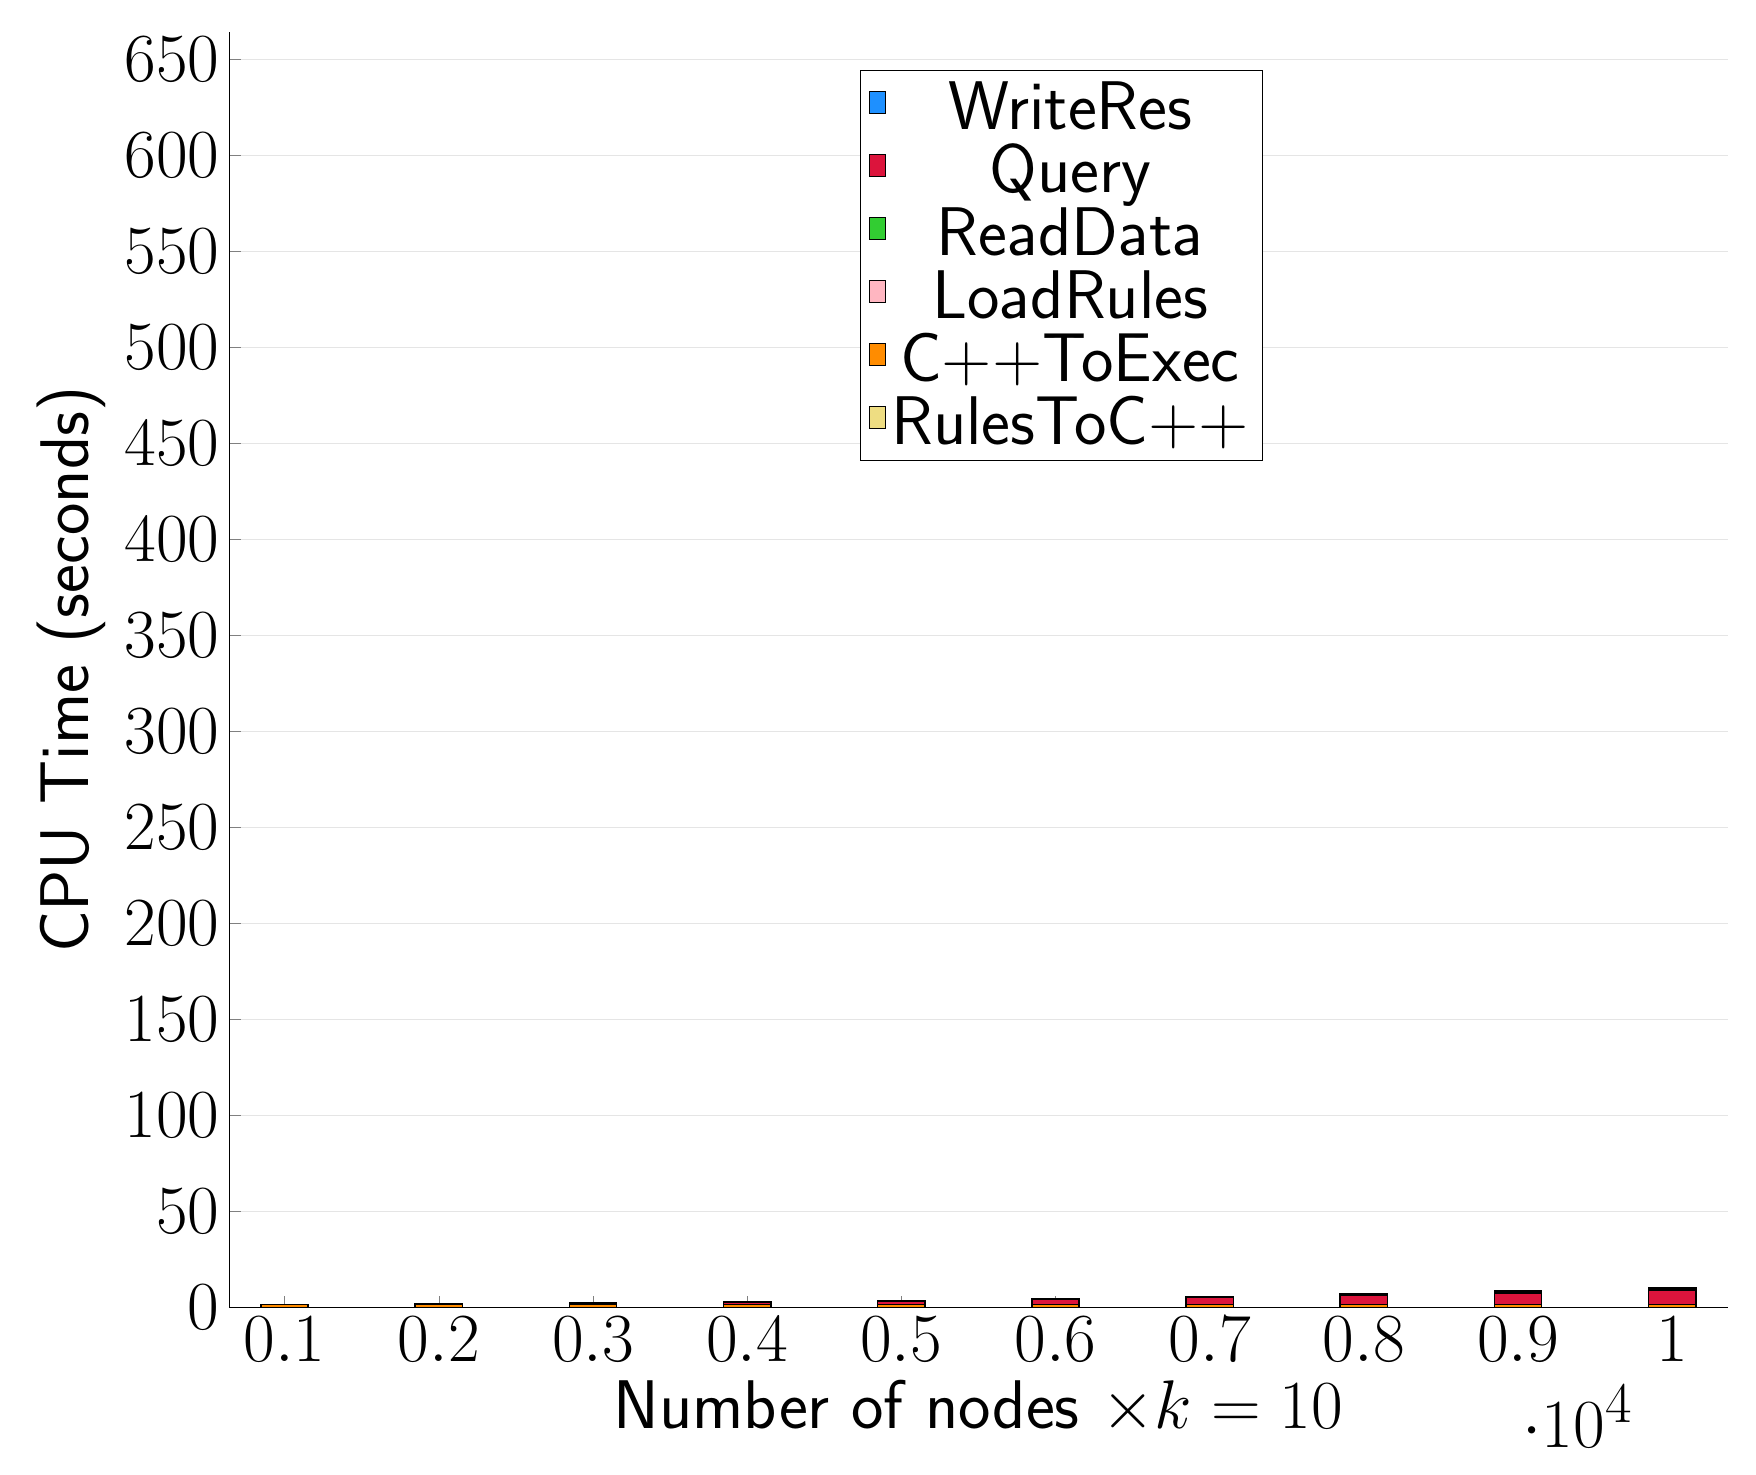
\begin{tikzpicture}
\begin{axis}[
   ybar stacked,
   width=1.7\textwidth,
   bar width=0.6cm,
   ymajorgrids, tick align=inside,
   major grid style={draw=gray!20},
   xtick=data,
   ymin=0, ymax=664.059,
   axis x line*=bottom,
   axis y line*=left,
   enlarge x limits=0.04,
   legend style={
       at={(0.69, 0.97)},
       anchor=north east,
       legend columns=1,
       font=\Huge,
   },
   ylabel={CPU Time (seconds)},
   xlabel={Number of nodes $\times k=10$},
   label style={font=\Huge},
   tick label style={font=\Huge},
]
\addlegendimage{fill=DodgerBlue, draw=black, line width=0.2pt}
\addlegendentry{WriteRes}
\addlegendimage{fill=Crimson, draw=black, line width=0.2pt}
\addlegendentry{Query}
\addlegendimage{fill=LimeGreen, draw=black, line width=0.2pt}
\addlegendentry{ReadData}
\addlegendimage{fill=LightPink, draw=black, line width=0.2pt}
\addlegendentry{LoadRules}
\addlegendimage{fill=DarkOrange, draw=black, line width=0.2pt}
\addlegendentry{C++ToExec}
\addlegendimage{fill=LightGoldenrod, draw=black, line width=0.2pt}
\addlegendentry{RulesToC++}
\addplot +[fill=LightGoldenrod, draw=black, line width=0.55pt] coordinates {
(1000, 0.0020000000000000005)
(2000, 0.0)
(3000, 0.008000000000000002)
(4000, 0.004000000000000001)
(5000, 0.006000000000000001)
(6000, 0.0020000000000000005)
(7000, 0.004000000000000001)
(8000, 0.003999999999999997)
(9000, 0.0020000000000000005)
(10000, 0.004000000000000001)
};
\addplot +[fill=DarkOrange, draw=black, line width=0.55pt] coordinates {
(1000, 1.464)
(2000, 1.4700000000000002)
(3000, 1.464)
(4000, 1.464)
(5000, 1.464)
(6000, 1.464)
(7000, 1.468)
(8000, 1.4740000000000002)
(9000, 1.47)
(10000, 1.4739999999999998)
};
\addplot +[fill=LightPink, draw=black, line width=0.55pt] coordinates {
(1000, 0.00016380000000000002)
(2000, 0.00015539999999999998)
(3000, 0.0001542)
(4000, 0.0001516)
(5000, 0.0001572)
(6000, 0.0001576)
(7000, 0.00015600000000000002)
(8000, 0.0001776)
(9000, 0.0001626)
(10000, 0.00016820000000000002)
};
\addplot +[fill=LimeGreen, draw=black, line width=0.55pt] coordinates {
(1000, 0.0039168)
(2000, 0.0074026)
(3000, 0.0103216)
(4000, 0.013134799999999999)
(5000, 0.0147482)
(6000, 0.017763400000000002)
(7000, 0.0203146)
(8000, 0.0219982)
(9000, 0.0223614)
(10000, 0.024902600000000004)
};
\addplot +[fill=Crimson, draw=black, line width=0.55pt] coordinates {
(1000, 0.0798616)
(2000, 0.2782822)
(3000, 0.6315489999999999)
(4000, 1.1465020000000001)
(5000, 1.811404)
(6000, 2.6391560000000003)
(7000, 3.6447720000000006)
(8000, 4.8037019999999995)
(9000, 6.141988)
(10000, 7.659197999999999)
};
\addplot +[fill=DodgerBlue, draw=black, line width=0.55pt] coordinates {
(1000, 0.0109124)
(2000, 0.0432664)
(3000, 0.098179)
(4000, 0.17308759999999998)
(5000, 0.270248)
(6000, 0.39185800000000004)
(7000, 0.526502)
(8000, 0.6883712)
(9000, 0.8682051999999999)
(10000, 1.064892)
};
\end{axis}
\end{tikzpicture}

\end{document}
